
\chapter{MOTION PRIMITIVE TRANSITION:WALK AND STANCE}
\label{chap:stance}
    \graphicspath{{WalkStance/WalkStanceFigs/EPS/}{WalkStance/WalkStanceFigs/}}

This chapter focuses on synthesizing transitional motions.
Another motion primitive:the stance is developed in Section~\ref{sec:stanceprimitive}.
The transitional motions from walking to stance and from stance to walking are discussed in Section~\ref{sec:transmotion}.




    
    




\section{The Stance Primitives}
\label{sec:stanceprimitive}
For passive walkers, if the walking velocity is not big enough after a  heel strike, the passive walker will stop walking and rest at the double support posture.
This stable posture is shown in Figure ~\ref{fig:bipedalstance}.
\begin{figure}[!htbp]
  \begin{center}
     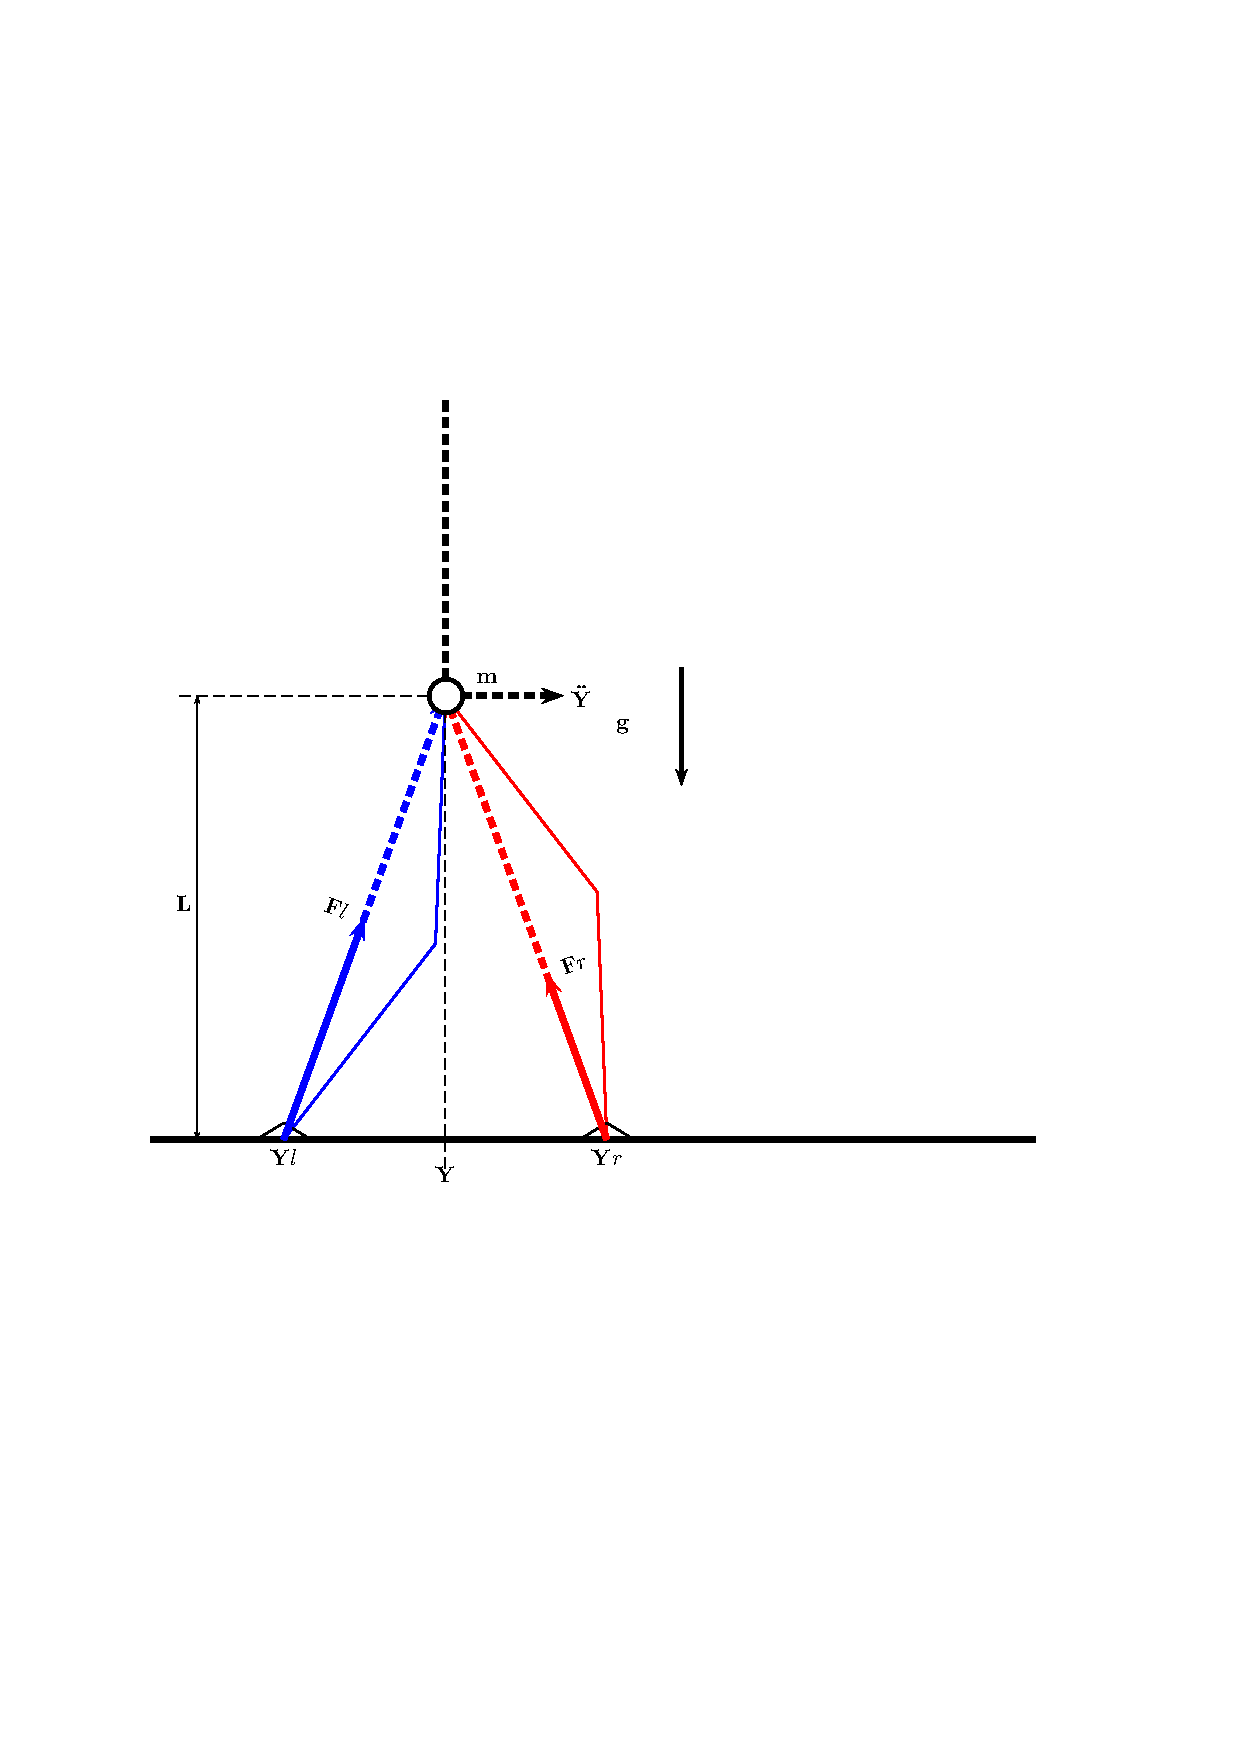
\includegraphics[width=0.7\textwidth]{stancefigure}
    \caption{The Stance Motion Primitives}
    \label{fig:bipedalstance}
\end{center}
\end{figure}

On phase plot, such motions have the topology of a fixed point attractor, which is  another motion primitive: the stance. 



\subsection{Simplified Dynamics}
When people stand, the two legs are almost straight.
Instead of the four linked rigid body model, the stance for this case can be simplified as a point mass supported by two straight legs. 
\citet{stephens2009modeling} proposed the height of waist is almost constant and can be neglected.
Therefore, the simplified dynamic model has only one degree of freedom, i,e. the horizontal displacement.
Given the horizontal displacement, configurations of shank and thigh can be worked out through \emph{inverse kinematic} methods.
 




The stance dynamic is not continues and the phase space can be divided into three regions.
The postures of different regions are shown in Figure~\ref{fig:phaseregionsofstance}.

\begin{figure}[!htbp]
  \begin{center}
     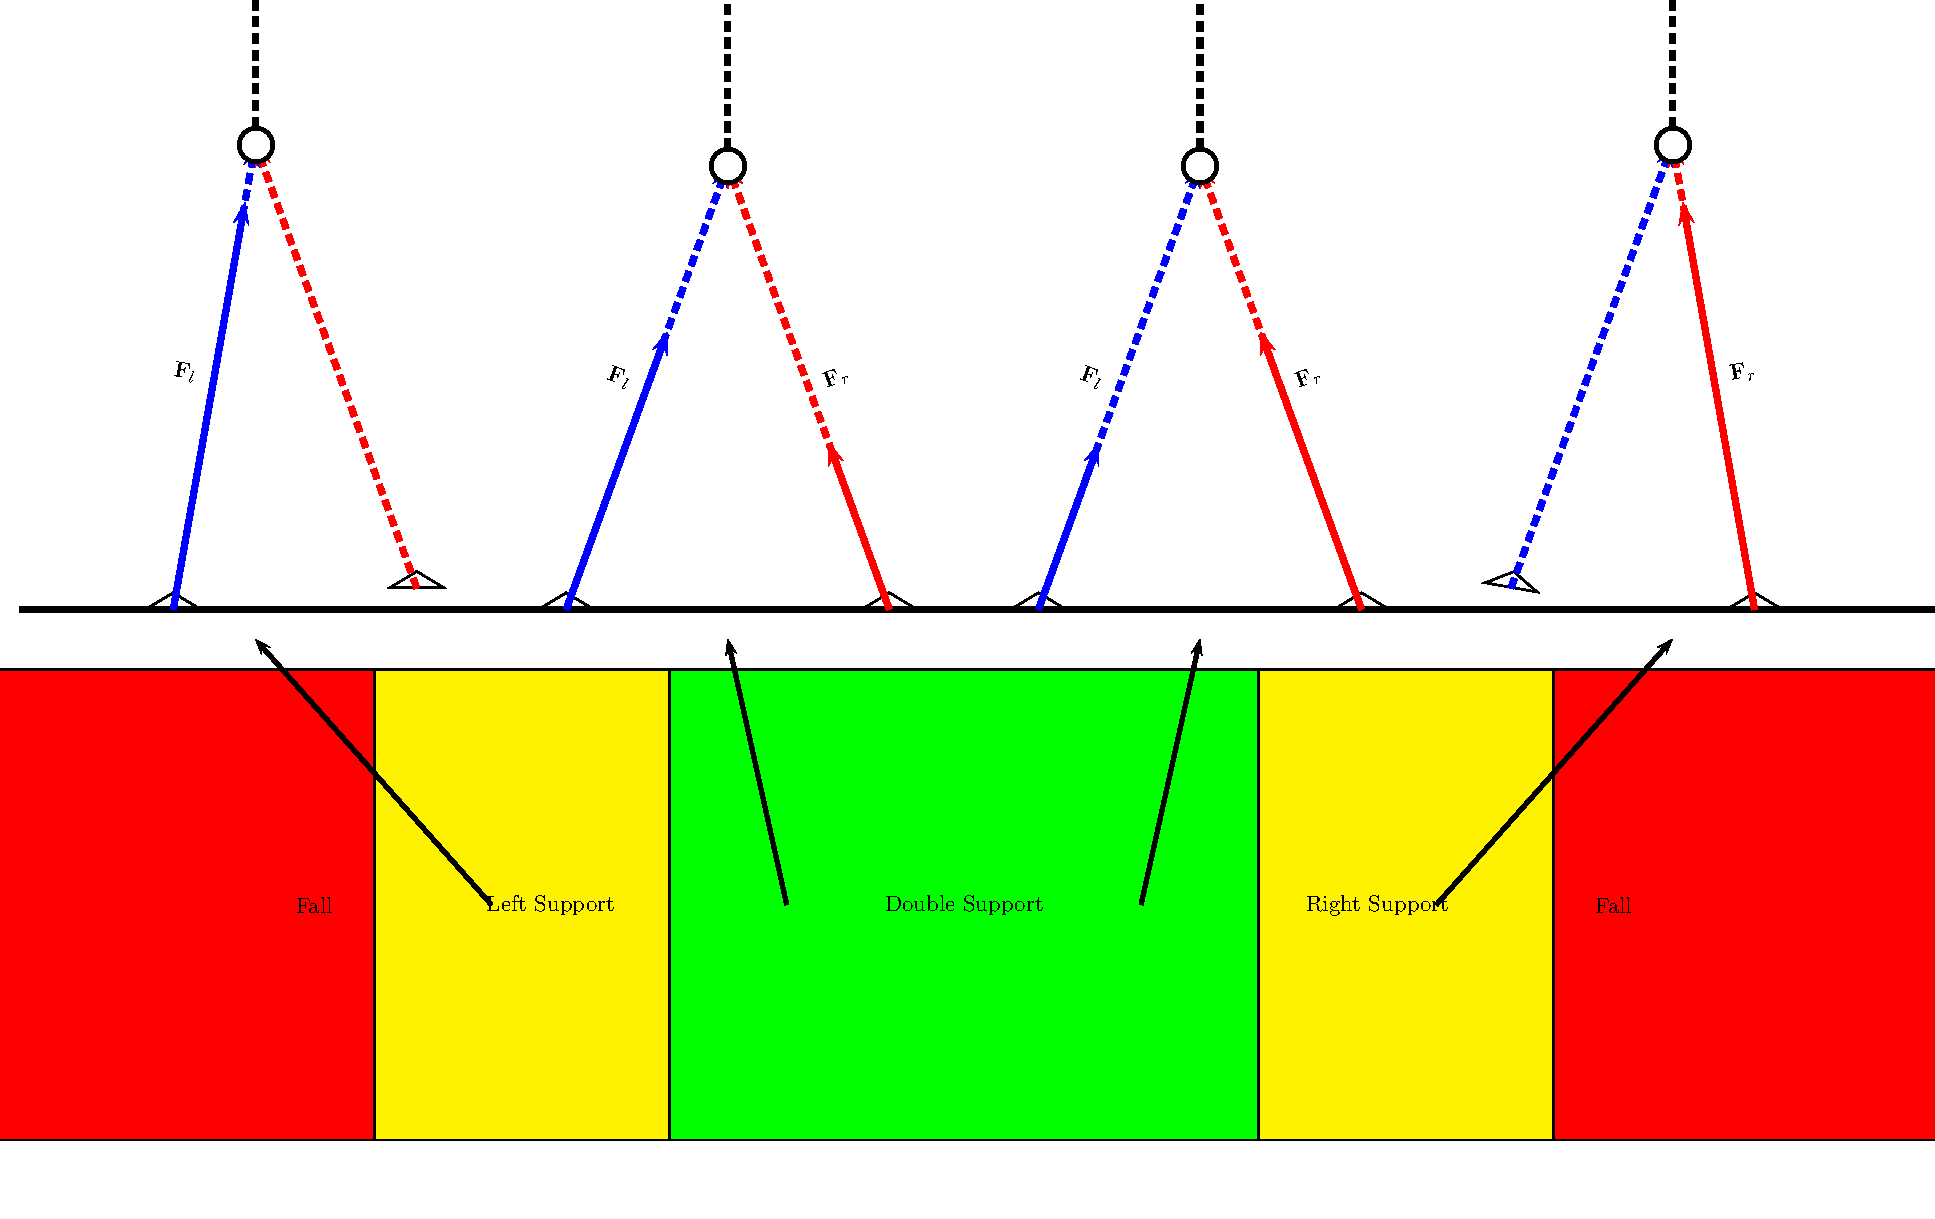
\includegraphics[width=0.7\textwidth]{stanceConfigure}
    \caption{discontinuous dynamics of stance}
    \label{fig:phaseregionsofstance}
\end{center}
\end{figure}


\begin{itemize}
\HiItem{Double Support}
When the off center  displacement  is small, the body is supported by two legs.
the motion is governed by the gravity.
\[
\ddot{q}=\frac{\gv}{L}(q-y_r)+\frac{\gv}{L}(q-y_l)
\]
where $q$ is the off center displacement,
$L$ is the height of the mass point, 
and $\gv$ is gravity.



Torques are generated by the two legs to maintain stability.
Intuitively, the left torque is increased when the centre moves left, and the same is true with the right torque.
We suppose the relationship between torques and centre position is linear.
Dynamic Equation~\ref{eq:stanceequation} incorporates the control strategy.
\begin{equation}
\label{eq:stanceequation}
\ddot{q}=\frac{\gv}{L}w_r(q-y_r)+\frac{\gv}{L}w_l(q-y_l)+\frac{\tau_L+\tau_R}{mL}
\end{equation}
where $w_l$ and $w_r$ are the weight of the two torques. 
We have $w_l+w_r=1$.


\HiItem{Single Leg Support}
For a big horizontal  displacement,  people stand on a single leg.
The passive dynamic is
\[
\ddot{q}=\frac{g}{L}q
\]
Equation~\ref{eq:singlestand} incorporates the torque generated by legs.
\begin{equation}
\label{eq:singlestand}
\ddot{q}=\frac{\gv}{L}q+\frac{y_{L,R}}{L}\tau_{L,R}
\end{equation}

\HiItem{Fall and Walk}
For even bigger displacement,  the stance posture can not be maintained.
The phase space region where human can maintain the stand posture is called ``support region''.
The width of the ``support region'' depends on the  height and the step size.
When moving out of the ``support region'', the stance posture can't be maintained, and a human will either walk or fall.
\end{itemize}







Without damping effects, the original system is similar to a mass spring system.
It will vibrate endlessly, and the flow is a circle, as shown in Figure~\ref{fig:stancepostures}.
If the speed is high, then the state will move out of the basin of attraction.
Maintaining stance is to maintain the horizontal displacement within the support region.
\begin{figure}[!htbp]
  \begin{center}
     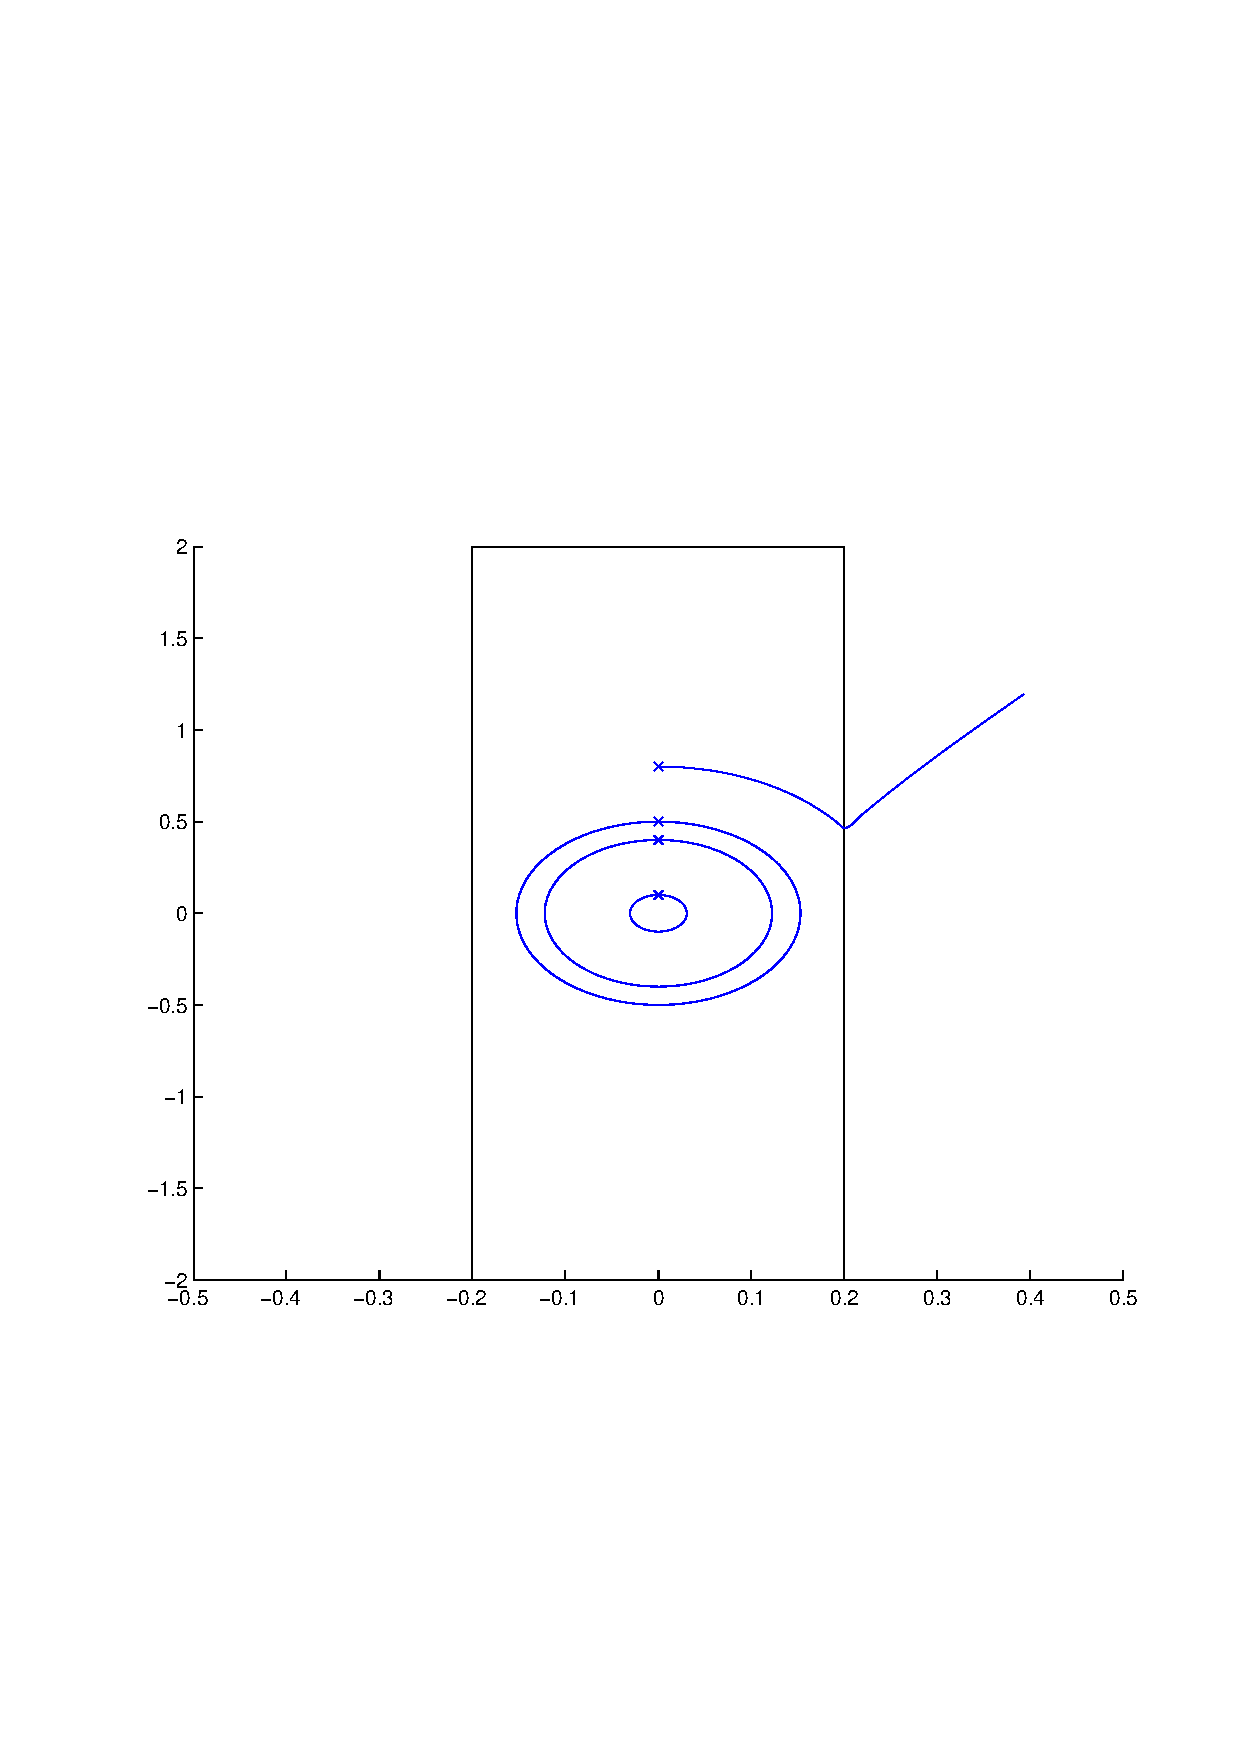
\includegraphics[width=0.7\textwidth]{uncontrolled}
    \caption{uncontrolled motion}
    \label{fig:stancepostures}
\end{center}
\end{figure}



\section {Motor Invariant Control}
\subsection{Entrainment}
By coupling the dynamic system with the neural oscillator, the position of the centre is fed into the neural oscillator and the output of the neural oscillator drives the torque generated by the legs.
\[
\uin=\hin(q)\\
\uout=\tau_{L,R}
\]
Entrainment happens and a limit cycle is formed.
However, since entrainment will no modify the boundary of the support region, entrainment does not boost the stability. 
It is impossible for mechanical system to converge to the limit circle within 1/4 period, and the neural oscillator will not modify the boundary.

\subsection{Local Invariant Control}
All the three group actions can be applied.
However, only two group actions among the three are useful and affect the stability.
\subsubsection*{Time Scaling}
Time scaling action will stretch the phase plot in the velocity direction, as shown in Figure~\ref{fig:stanceTimeScaling}.
It will enlarge the basin of attraction to include high speed state.
\begin{figure}[!htbp]
  \begin{center}
      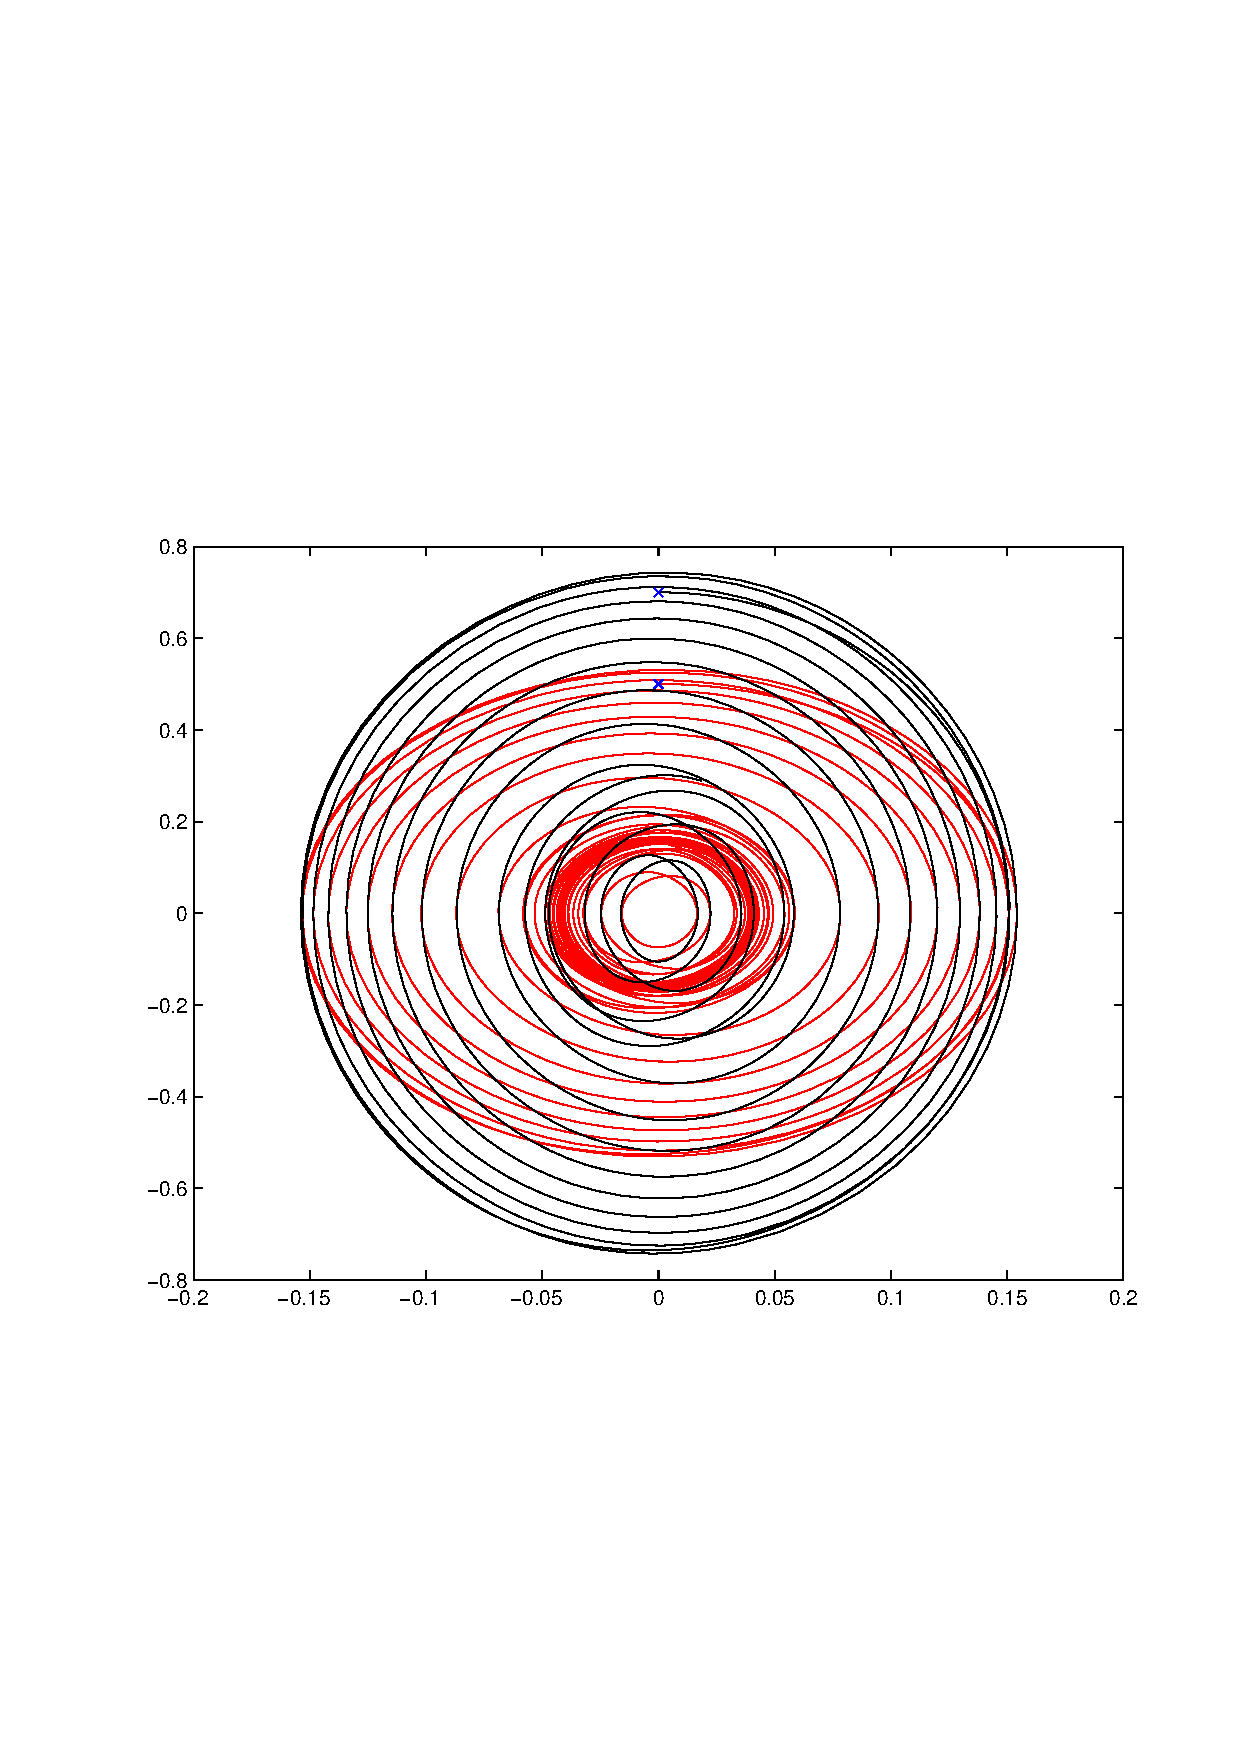
\includegraphics[width=0.7\textwidth]{TimeScaling}
    \caption{Time Scaling}
    \label{fig:stanceTimeScaling}
\end{center}
\end{figure}



\subsubsection*{Energy Control}
Energy scaling action will modify the size of the limit cycle, which modifies the wobbling amplitude.
Figure~\ref{fig:energyscaling} shows the energy action effect on the limit cycle.
When energy action is applied, the limit cycle shrinks.


\begin{figure}[!htbp]
  \begin{center}
      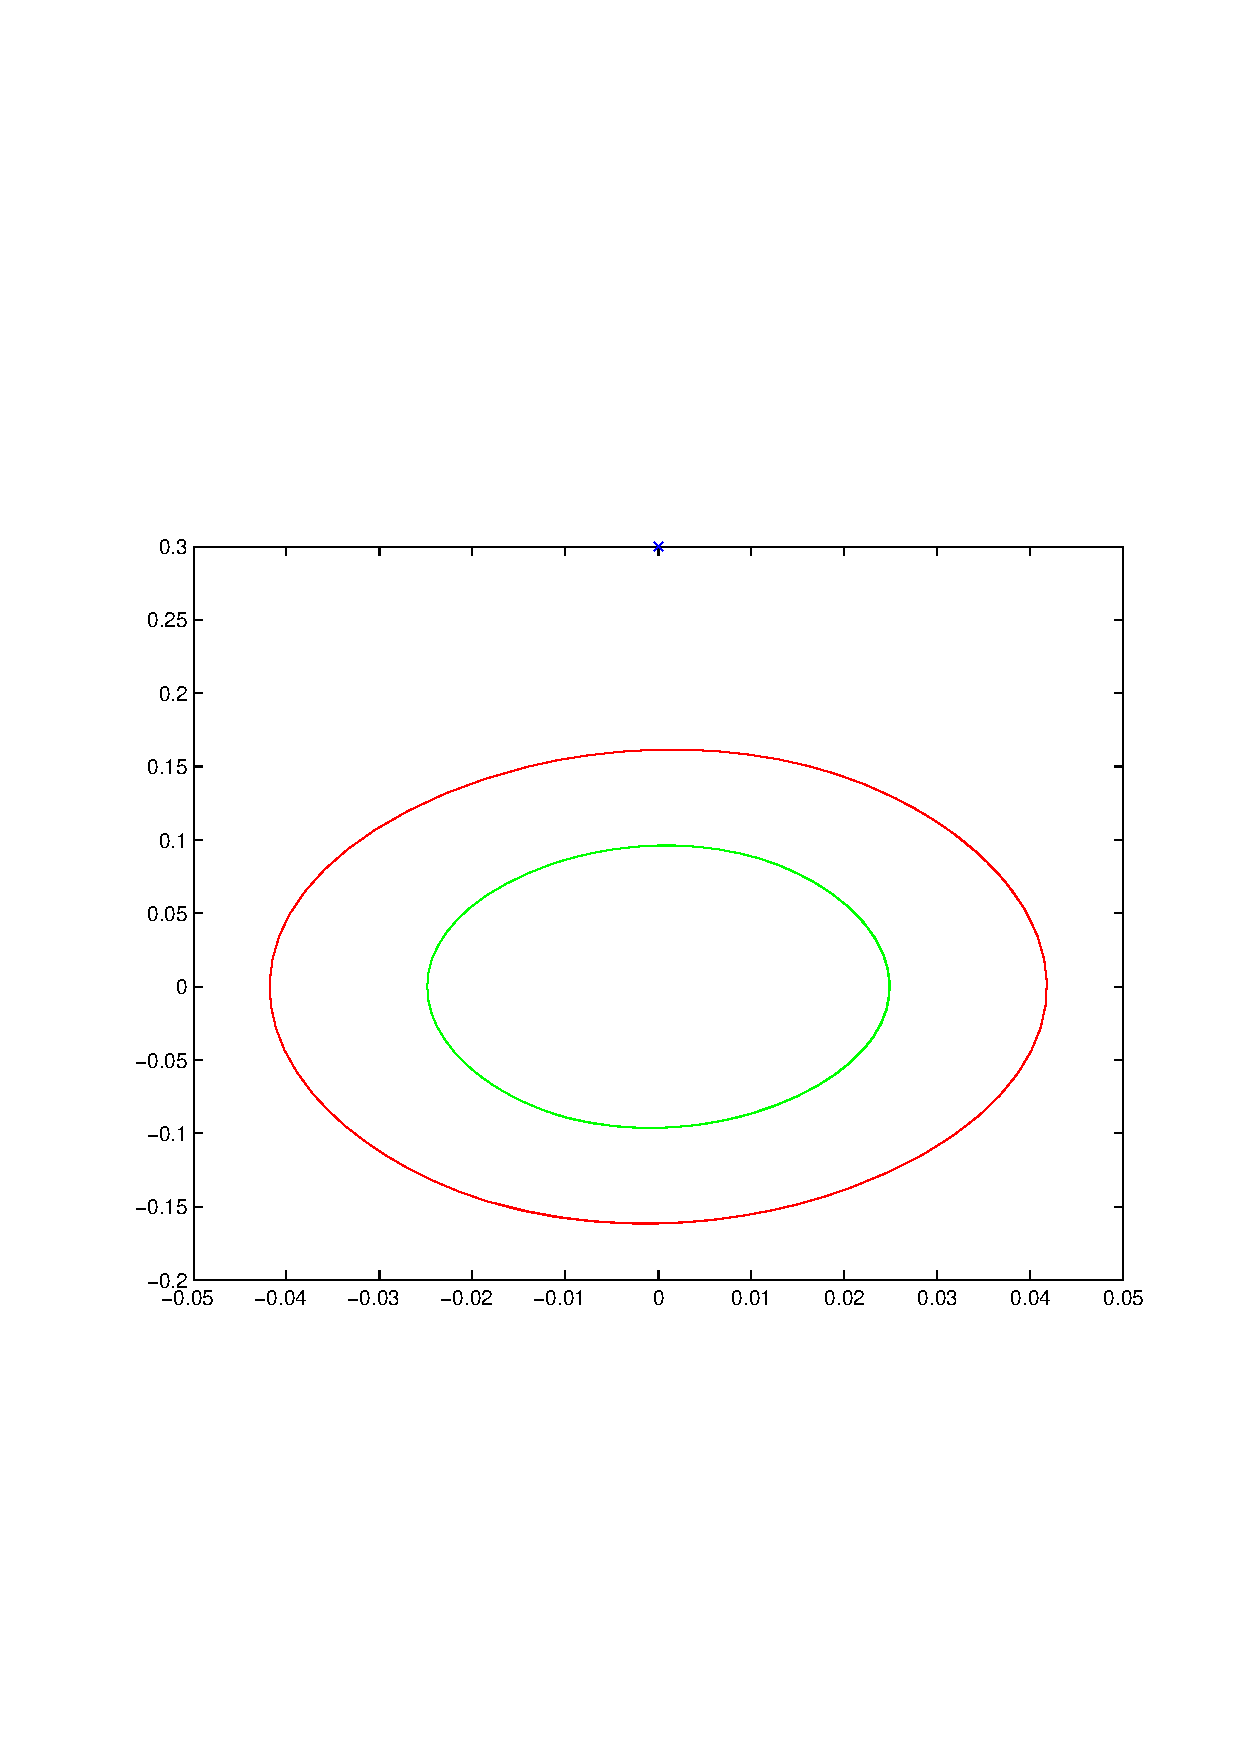
\includegraphics[width=0.7\textwidth]{EnergyControlled}
    \caption{Energy Scaling}
    \label{fig:energyscaling}
\end{center}
\end{figure}





\subsubsection*{Fast Convergence Control}
By applying speed and energy scaling actions sequentially, wobbling can converge to the limit cycle and stop quickly.
In Figure ~\ref{fig:fastconverg}, the speed action is first applied to include the high speed state for 1/4 period. 
When the state reach the pos that the speed is zero, the energy scaling is applied for next $1/4$ period to shrink the limit cycle size.
For the next $1/4$ period,  the speed action is applied, and so on.

\begin{figure}[!htbp]
  \begin{center}
      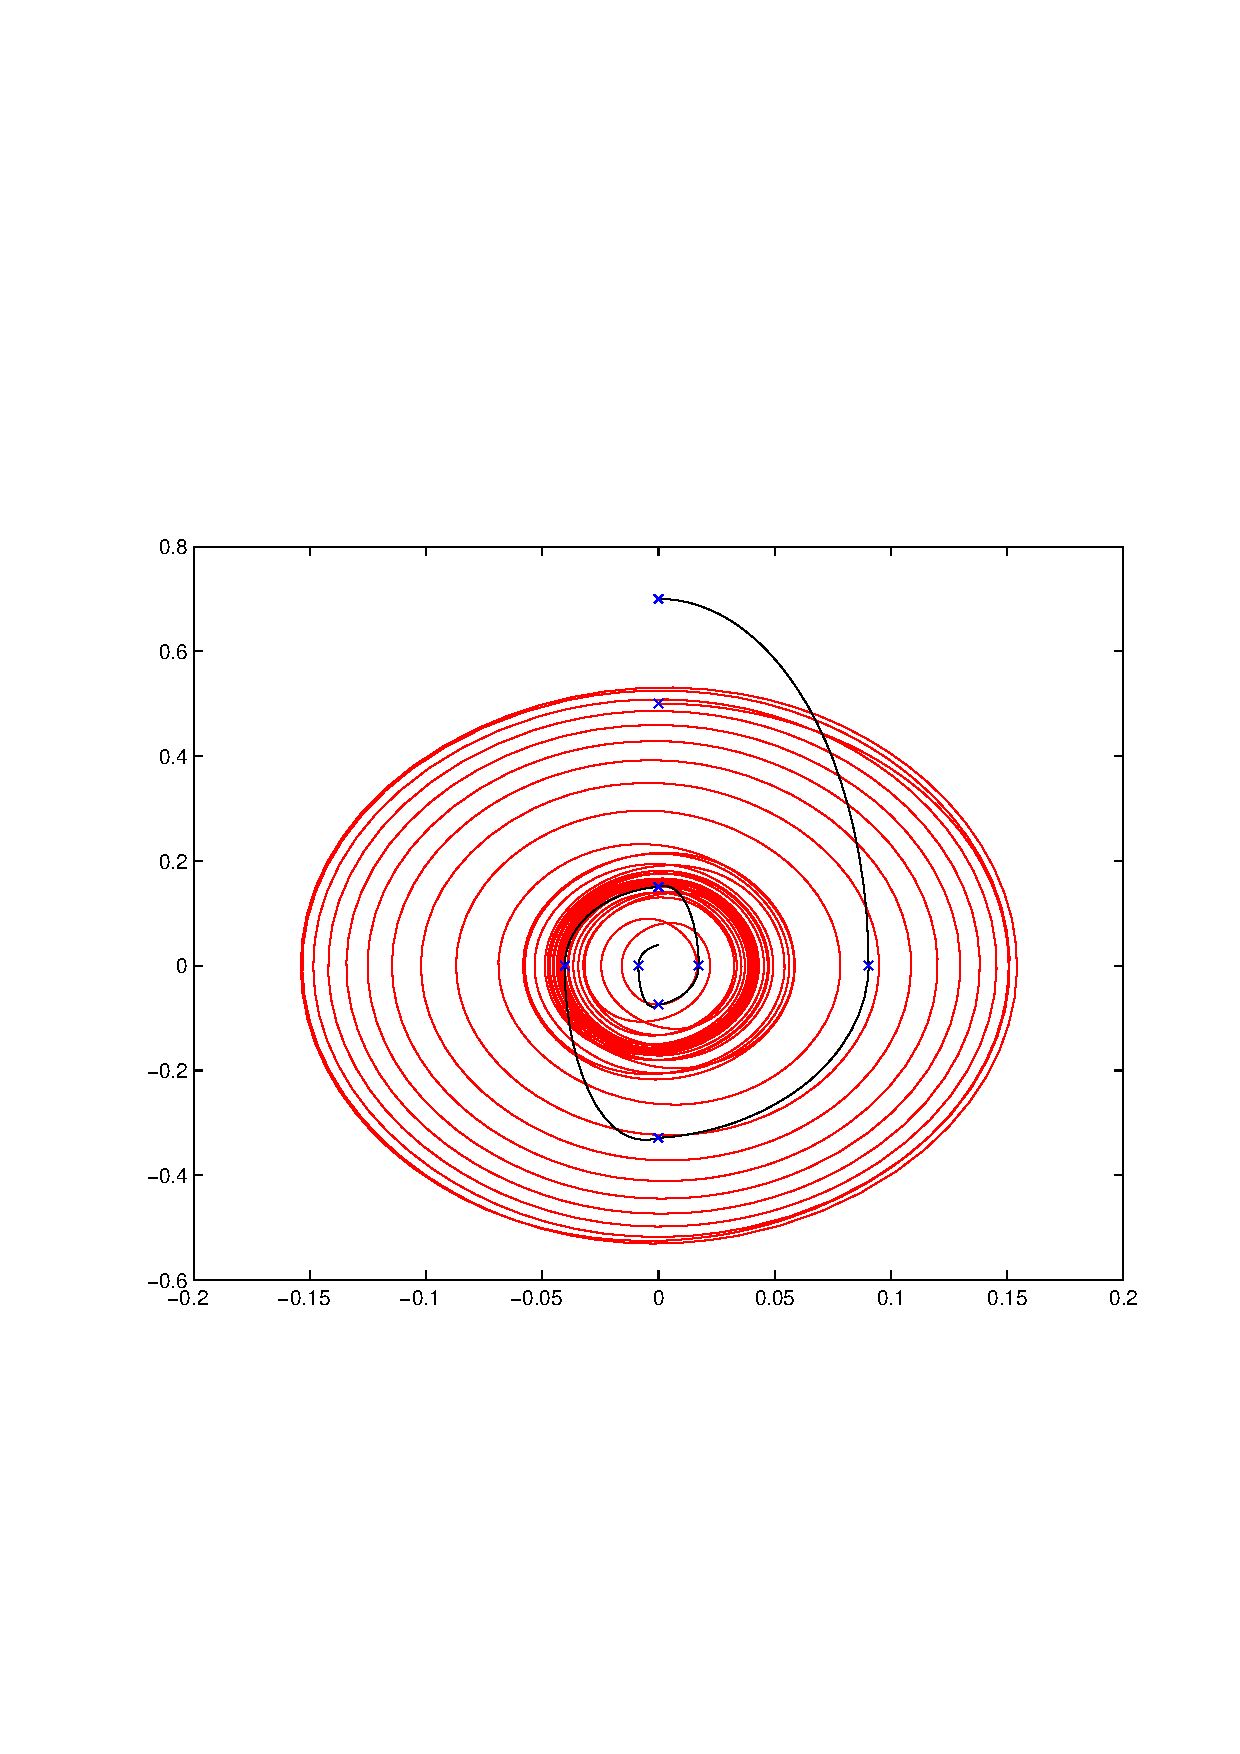
\includegraphics[width=0.7\textwidth]{FastCoverge}
    \caption{Fast Converge}
    \label{fig:fastconverg}
\end{center}
\end{figure}

\subsection{Stability}
Motions of stance are put together for comparison.
Without any control, the character fails as shown in Figure~\ref{fig:stancefall}.
\begin{figure}[h]
\begin{center}$
\begin{array}{ccccc}
\includegraphics[width=1in]{stanceFall/0001.eps}&
\includegraphics[width=1in]{stanceFall/0021.eps}&
\includegraphics[width=1in]{stanceFall/0041.eps}&
\includegraphics[width=1in]{stanceFall/0061.eps}&
\includegraphics[width=1in]{stanceFall/0081.eps}
\\
\includegraphics[width=1in]{stanceFall/0101.eps}&
\includegraphics[width=1in]{stanceFall/0121.eps}
\end{array}$
\end{center}
\caption{Balance Motion without Neural Control}
    \label{fig:stancefall}
\end{figure}

In Figure~\ref{fig:stancespeed}, the speed action is applied, and the character maintains its stance motion, but wobbles endlessly.
\begin{figure}[!htbp]
  \begin{center}
  $
     \begin{array}{ccccc}
\includegraphics[width=1in]{stancewobble/0001.eps}&
\includegraphics[width=1in]{stancewobble/0021.eps}&
\includegraphics[width=1in]{stancewobble/0041.eps}&
\includegraphics[width=1in]{stancewobble/0061.eps}&
\includegraphics[width=1in]{stancewobble/0081.eps}
\\
\includegraphics[width=1in]{stancewobble/0101.eps}&
\includegraphics[width=1in]{stancewobble/0121.eps}&
\includegraphics[width=1in]{stancewobble/0141.eps}&
\includegraphics[width=1in]{stancewobble/0161.eps}&
\includegraphics[width=1in]{stancewobble/0181.eps}

\end{array}$
    \caption{Wobbling Stance}
    \label{fig:stancespeed}
\end{center}
\end{figure}

In Figure~\ref{fig:fastconverge}, both speed action and energy action are applied, and the character maintains the stance and  vibrates with a shrinking amplitude.
\begin{figure}[!htbp]
  \begin{center}
        $\begin{array}{ccccc}
\includegraphics[width=1in]{stanceconverge/0001.eps}&
\includegraphics[width=1in]{stanceconverge/0021.eps}&
\includegraphics[width=1in]{stanceconverge/0041.eps}&
\includegraphics[width=1in]{stanceconverge/0061.eps}&
\includegraphics[width=1in]{stanceconverge/0081.eps}
\\
\includegraphics[width=1in]{stanceconverge/0101.eps}&
\includegraphics[width=1in]{stanceconverge/0121.eps}&
\includegraphics[width=1in]{stanceconverge/0141.eps}&
\includegraphics[width=1in]{stanceconverge/0161.eps}&
\includegraphics[width=1in]{stanceconverge/0181.eps}

\end{array}$
    \caption{Stable Stance}
    \label{fig:fastconverge}
\end{center}
\end{figure}




\section{Walking and Stance Transition}
\label{sec:transmotion}
Both limit cycles of walking and stance are shown in Figure~\ref{fig:walksstance}.
The phase plot here shows the supporting leg, and the swing leg is indicated in shadow red.
Motion transition means make the state transform from one limit cycle into another.





\subsection{Walk to Stance}
Walk to stance transition happens at the heel strike phase.
Without control effort, the bipedal machine will continue to walk.
As shown in Figure~\ref{fig:walksstance}, if we switch on the stance motion primitive controller, the current state will fall into the basin of attraction of stance with a proper group transform action. 
Two legs will vibrate with smaller amplitude, this is the walk to stance transition.

\begin{figure}[!htbp]
  \begin{center}
    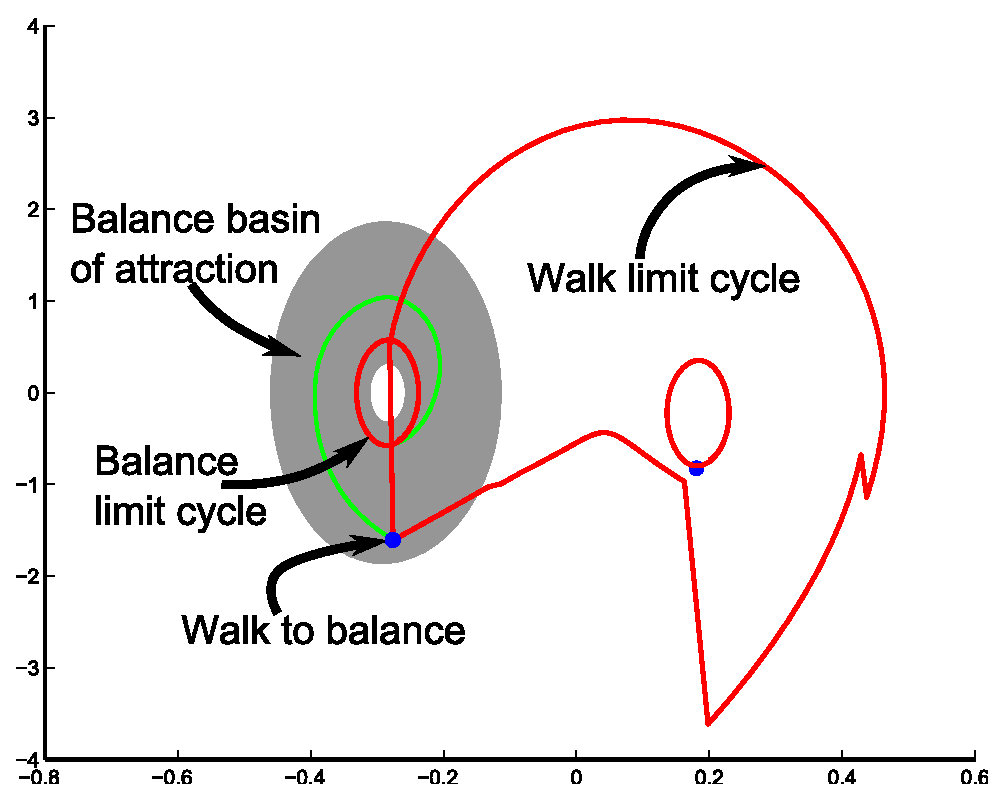
\includegraphics[width=0.7\textwidth]{walk_to_stand}
    \caption{Fast Converge}
    \label{fig:walksstance}
	\end{center}
\end{figure}



%\begin{figure}[!htbp]
%  \begin{center}
%      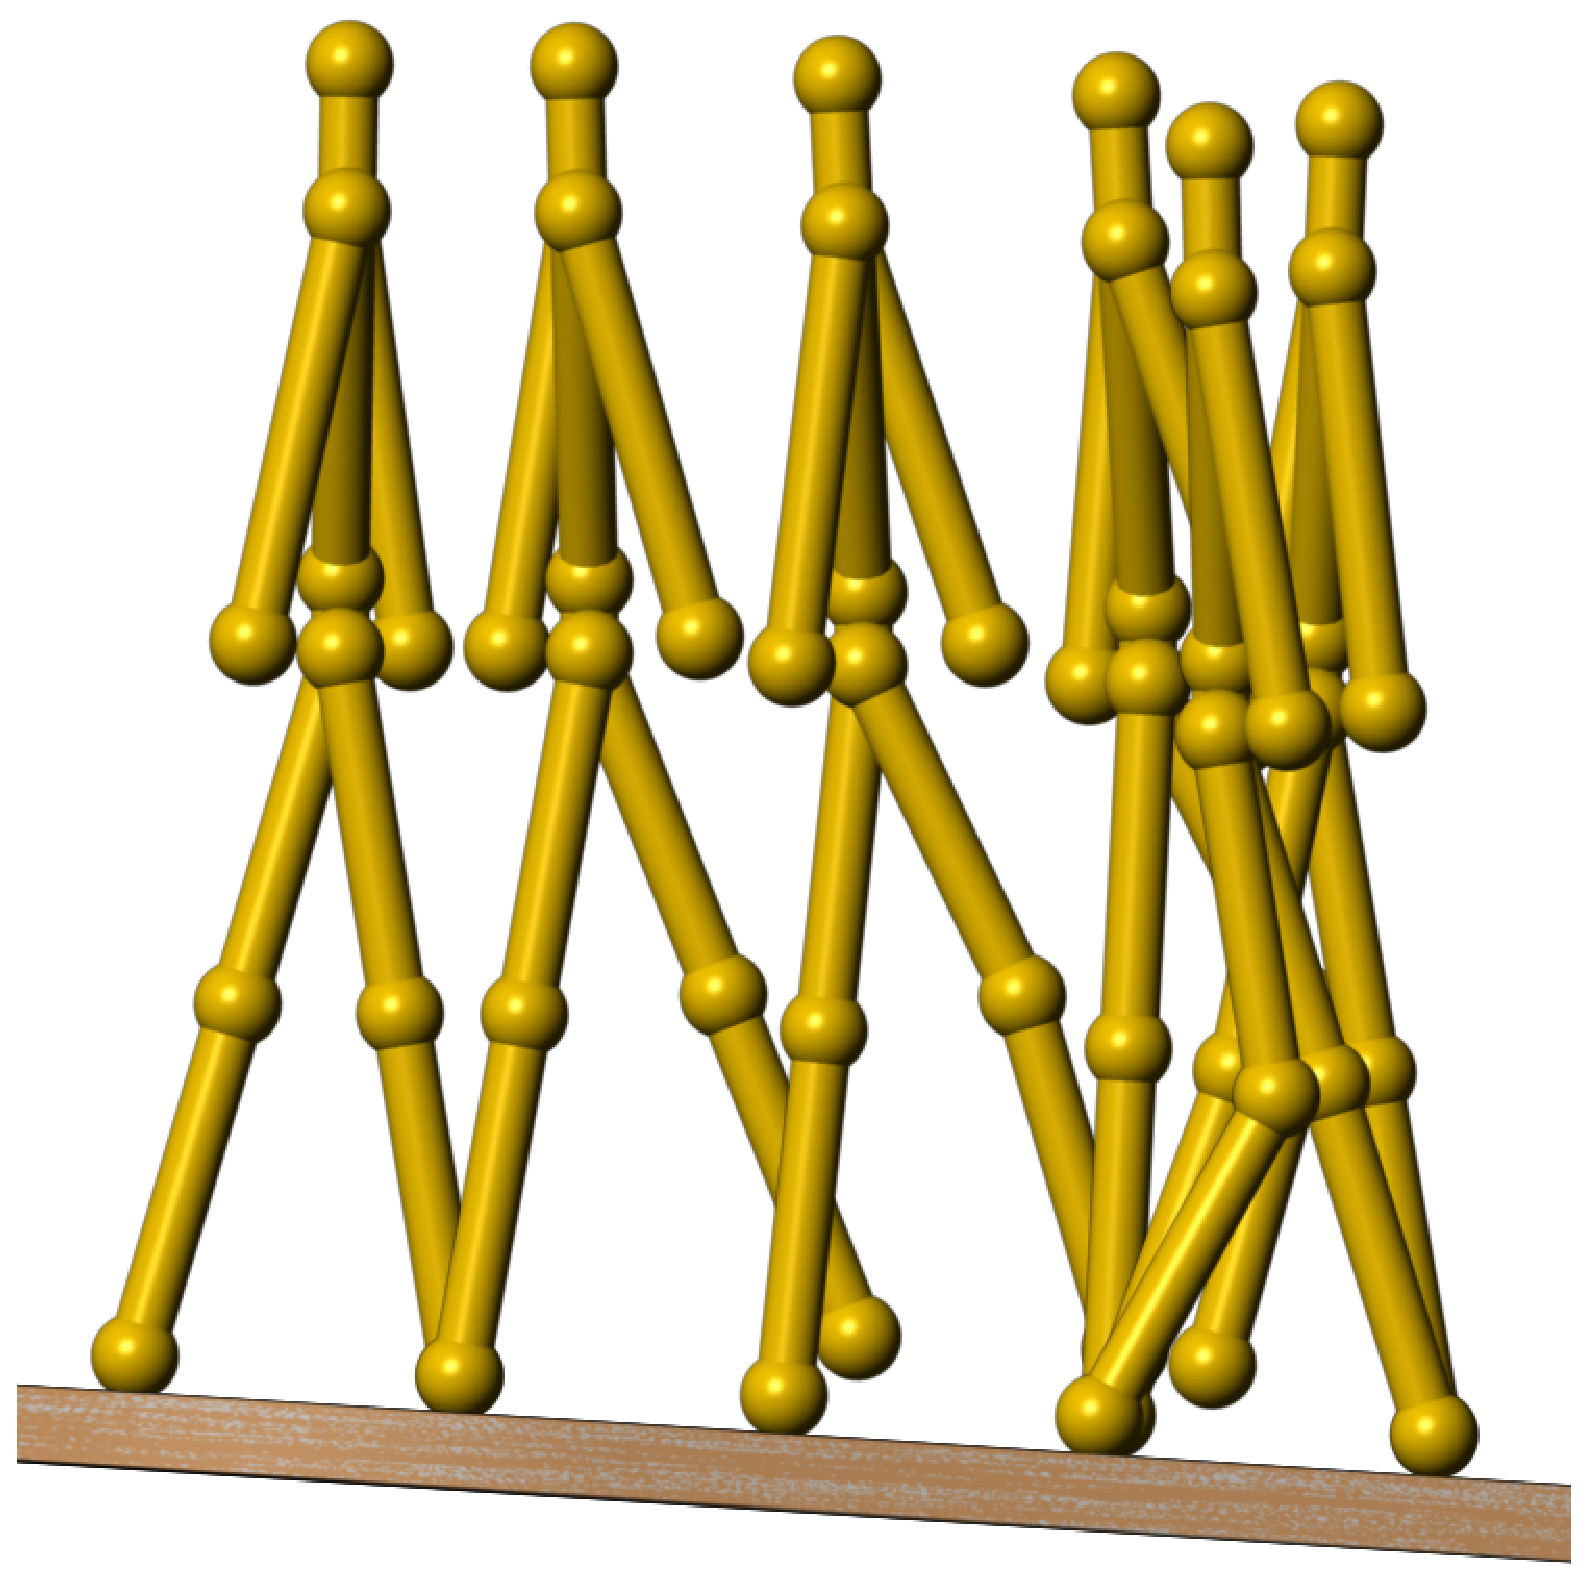
\includegraphics[width=0.7\textwidth]{walk_to_balance}
%    \caption{Walk to Balance}
%    \label{fig:walk2stance}
%\end{center}
%\end{figure}




\subsubsection*{Knee Bending Scheme}
During walk to stance transition, the two legs are straight when the heel strikes.
Any push of the figure, it will move out of the two support regions. 
At this time, the support region is very small.
Any push of the figure, it will move out of the two support region.
To enlarge the basin of attraction, the walkers have to bend legs and lower the height.
There are many ways for bending the legs.


\begin{itemize}
	\HiItem{One Leg Bending}
		walker can bend one leg while keeping the other leg straight.
	\HiItem{Double Leg Bending}
		walker can make the two leg bend.
\end{itemize}
Since the knees is not necessary straight when a human walk, it is very difficult to tell which one is more realistic. 
These two schemes are extreme cases.
Motion of Double Leg Bending  is shown in Figure~\ref{fig:walkstancestraight}.
\begin{figure}[!htbp]
  \begin{center}
$\begin{array}{ccccc}
\includegraphics[width=1in]{WalkStanceTransition/0001.eps}&
\includegraphics[width=1in]{WalkStanceTransition/0101.eps}&
\includegraphics[width=1in]{WalkStanceTransition/0201.eps}&
\includegraphics[width=1in]{WalkStanceTransition/0301.eps}&
\includegraphics[width=1in]{WalkStanceTransition/0401.eps}
\\
\includegraphics[width=1in]{WalkStanceTransition/0501.eps}&
\includegraphics[width=1in]{WalkStanceTransition/0601.eps}&
\includegraphics[width=1in]{WalkStanceTransition/0701.eps}&
\includegraphics[width=1in]{WalkStanceTransition/0801.eps}&
\includegraphics[width=1in]{WalkStanceTransition/0901.eps}
\end{array}$    
    \caption{Stop Walking with Two Legs Bend}
    \label{fig:walkstancestraight}
\end{center}
\end{figure}



\subsection{Stance to Walk}
When the stance to walk transition happens,the current state should  be close to the walking limit cycle.
Due to this reason, stance to walk happens when the legs are moving forward at maxim speed and the position of the hip is in the middle.
At this time, we switch on the walker controller, and the character starts walking.
Figure~\ref{fig:stance2walk} shows the process on phase plot.
\begin{figure}[!htbp]
  \begin{center}
     \includegraphics{stance2walk}
    \caption{The Phase Plot for Stance to Walk}
    \label{fig:stance2walk}
\end{center}
\end{figure}


From stance to walk, the height has to be increased.
Only one scheme exists for straightening the knees.
The scheme which we use is to keep the front leg straight and make the hind leg from bend to straight.


Another non-trivial problem is is that when switching stance to walk, it is impossible to put both legs on the limit cycle.
The supporting leg has been given the priority, for the supporting leg is more important for maintaining stability.





\subsection{Smooth Transition by  Speed Action}
When transiting from walk to stance, the basin of attraction must include the heel strike state.
However, the original basin of attraction of stance does not. 
A speed action is needed to enlarge the basin of attraction.
As an alternative, we can lower the walker speed. 
In this way, walking to stance may become easier.

For the transition from stance to walk, if little effort is exerted, the initial position will be far from the walking limit cycle.
To maintain the walking stability, speed actions are applied to decrease the walking speed.

To make both limit cycles connected each other, the speed action of stance and walking mus have a constant ratio,
This phenomenon is common for our daily experience.
Here we give it a mathematical meaning.

























